\documentclass[a4paper,11pt]{article}
\usepackage[T1]{fontenc}
\usepackage[utf8]{inputenc}
\usepackage{lmodern}
\usepackage{amsmath}
\usepackage{graphicx}


\title{Smart Phone Cryptography: A comparison of techniques for encrypted data communication \\ Progress Report}
\author{Tom Nicholls}

\begin{document}

\maketitle

In this progress report document details will be given as to how this project has evolved from the description presented in the project specification, outlining and justifying any changes made. The state in which the project is currently in will be shown, including a presentation of the work completed up to this point. This will included any design and project choices that have been made. The document will be finished with a detailed plan of how the project will continue over the next term, up to completion. 

\section{Project Alterations}

Since the project specification document, this project has undergone a few changes in order to ensure that it is both an interesting project and also that it includes sufficient original work and accomplishments to current areas of Computer Science. This section details the adjustments made to the project.

\subsection{The Problem Definition}  

The main alterations in this project can be best described through a statement of the new problem definition:

The privacy of sensitive information has always been an important issue. With the increased popularity and usability of smart phones, tasks from accessing confidential work files or personal bank accounts to communicating with clients and friends, are being completed through applications over mobile, wireless internet connections. 

In this project I will research the various cryptographic schemes used by popular applications available to smart phones running the Android operating system for secure data transmission and communication. Accompanying this research will be a study and comparison of other schemes which could be used instead of those presented previously. A currently used cryptographic technique and an alternative technique will be implemented through a data transmission application. Tests will be carried out to analyse various important factors that need to be considered for a successful encrypted data transmission application, such as mobile data usage or cryptanalytic methods required to break the data encryption. An original conclusion will then be drawn as to whether the current techniques of cryptography available are appropriate or if a new scheme should be encouraged. How this conclusion can be extended to encompass functions other than text transmission will then be presented, for instance secure secret sharing.

\subsection{Objectives}

To further explain the adjustments made, the new objectives of the project will be presented.

\paragraph{Main Objectives}
\begin{enumerate}
  \item Research
  \begin{itemize}
    \item Framework design
    \item Cryptographic Techniques
    \item Currently Available Applications
    \item Relevant factors that can be used to compare schemes implemented on a mobile device
  \end{itemize}
  \item Implementation
  \begin{itemize}
    \item Framework
    \begin{itemize} 
      \item Design Data Communication framework
      \begin{itemize}
        \item Server
        \item Mobile Application
        \item P.C Client
      \end{itemize}
      \item Build, test and document framework
    \end{itemize}
  \item Encrypted Data Communication
  \begin{itemize}
    \item Design and implement cryptographic techniques, justifying choices
    \item Test and document implementation
  \end{itemize}
  \end{itemize}
  \item Analysis
  \begin{itemize}
    \item Perform tests from research
    \item Collect and present results
  \end{itemize}
  \item Conclusion
  \begin{itemize}
    \item Present and justify the findings and conlusions that can be made form the completed tests
    \item Show possible adjustments to the implemented schemes which would increase their usability
  \end{itemize}
  \item Further Work
  \begin{itemize}
    \item Detail possible extensions that can be made to the systems to include other possible functions
  \end{itemize}
  \item Documentation
  \begin{itemize}
    \item Design documentation layout
    \item Complete and proof read full documentation
  \end{itemize}
\end{enumerate}

\paragraph{Secondary Objectives}
\begin{enumerate}
  \item Design, create and justify an industry acceptable and marketable user interface for the finished product
  \item Implement functionality described in the further work objective (Objective 5)
\end{enumerate}

\subsection{Additional Changes}

Aside from the adjustments made in the problem definition and objectives sections detailed above, only minimal changes have been made to the rest of the project specification. For example in the 'Methods' section the research phase can still be completed in parallel to the framework development phase, with all other objectives requiring the objective before it to be completed before it can be started. Furthermore, only minor changes been made to the 'Resources' section; re-wording of the project components to account for the changes mentioned above and the addition of the Google application market place 'Google Play' to the list of resources. This is available through the internet which I have full access to.

A final addition to the specification that should be noted is the inclusion of another legal issue surrounding the project. As the resulting product of this project facilitates the secure and secret communication of messages which, in the wrong hands, could be used to aid a number of illegal operations such as crime organisation or terrorism. To avoid this issue in a legal sense I will not publish the final application to the Google market place and I will also present a legal disclaimer attached to this product incase someone does obtain a copy of the application. The issue could also be viewed as an ethical issue, but the actions taken to escape the legal issue should ensure the avoidence of the issue viewed in an ethical sense. 

\section{Work Completed}

In this section the work that has been completed in this project so far will be presented.

\subsection{Research}

In this project, the first task was to perform research (see Objectives section). An overview of the results of the research performed is described below. The results of this research will be formally presented and described in more detail in the final project report.

\begin{enumerate}
  \item
  \begin{description}
    \item[Framework Design] 
  \end{description}
  Research was made into how a system could be set up to facilitate the communication of data messages between any two users of the system. The result of this research, to utilise a multi-client server, can be found in the design section, where an outline of the system to be created is given.
  \item
  \begin{description}
    \item[Cryptographic Methods] 
  \end{description}
  \item
  \begin{description}
    \item[Current Applications] 
  \end{description}
  As a result of searching on the Google application marketplace ‘Google Play’, only two different applications currently exist that perform encrypted message communication. These two applications are:
  \begin{itemize}
    \item RSA Cipher Cat by Miasoft
    \item Cloak SMS Free by Hamish Medlin
  \end{itemize}
  Both applications allow the communication of encrypted messages between two users of the application. RSA Cipher Cat utilises the RSA asymmetric encryption scheme whereas Cloak SMS Free is uses the AES symmetric key encryption scheme.
  \item
  \begin{description}
    \item[Mobile device application comparison factors] 
  \end{description}
  As the third section of this project is concerned with the analysis and comparison of cryptographic schemes, research was performed to discover which factors impact how successful and useful an encryption scheme on a mobile device is. The discovered factors are:
  \begin{itemize}
    \item Difficulty of techniques required to break encryption
    \item Energy Consumption/Battery power required
    \item Operation and Processing Time
    \item Cryptographic key size
    \item Mobile data usage
    \item Application size
    \item Number/Duration of data connection required
  \end{itemize}
\end{enumerate}

\subsection{Design}

As can be seen from the previous sections in this document, this project includes a software development section. The system is built upon a multi-client server facilitating the communication of data between two clients.  This data is encrypted (and decrypted) using different cryptographic schemes.

\begin{figure}[htb]
\centering
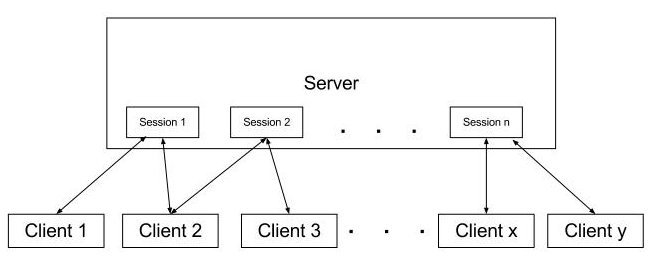
\includegraphics[scale=0.35]{designs1.jpg}
\caption{The server can create many communication sessions from a collection of clients}
\label{fig:designs1}
\end{figure}

The server creates a session between two clients that wish to communicate. Clients initiate sessions with any client with which they have shared their indentification code (ID number). Each session is a new thread within the server. This allows the server to establish any number of sessions, to allow for multiple communication links between any two clients. As can be seen in Figure \ref{fig:designs1}, any client can have more than one communication session at any one time, with any other client in the client base.

\begin{figure}[htb]
\centering
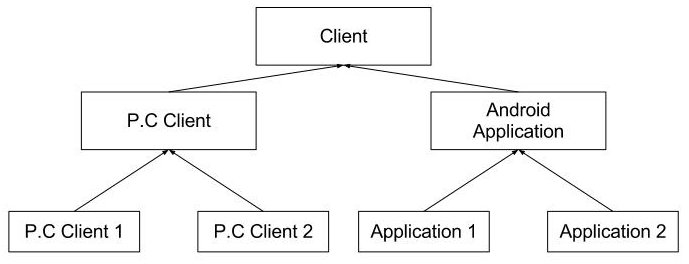
\includegraphics[scale=0.35]{designs2.jpg}
\caption{Inheritance properties of the clients}
\label{fig:designs2}
\end{figure}

Communication between two clients is facilitated via the server. A client can be either a P.C client or an Android Application (client) allowing data to be sent between these two mediums. Compatibility between the clients will be ensured through the use of the XML file structure. For example, if two cryptographic schemes are implemented; Application 1 and P.C Client 1 will utilise scheme 1 and Application 2 and P.C 2 will utilise scheme 2. This can be easily achieved due to the usage of the model in Figure~\ref{fig:designs1}. The main Android Application sends unencrypted data to the server and receives unencrypted data back. Application 1 (and 2) inherits these features, with the ability to add in their respective methods for encryption. This is the same for the P.C clients.

\begin{figure}[htb]
\centering
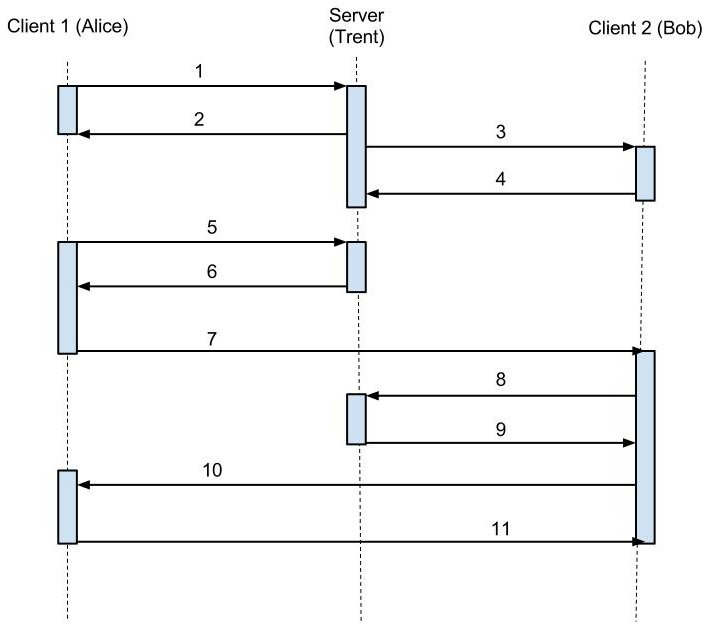
\includegraphics[scale=0.35]{designs3.jpg}
\caption{Sequence diagram showing distribution of public keys}
\label{fig:designs3}
\end{figure}

The encryption schemes used within this project all require the sharing of public keys. Figure~\ref{fig:designs3} shows how this will be achieved. The placeholder names ‘Alice’, ‘Bob’ and ‘Trent’ have been used following the tradition set out in most cryptography materials.

\begin{enumerate}
  \item Alice registers her public key $ K_{A} $ with Trent
  \item Trent sends his public key $ K_{T} $ to Alice
  \item Bob registers his public key $ K_{B} $ with Trent
  \item Trent sends his public key $ K_{T} $ to Bob
  \item Alice sends to Trent: $ Alice, Bob, Timestamp1 $
  \item Trent sends to Alice: $ \{K_{B},Bob, Timestamp1\} K_{T}^{-1} $
  \item Alice checks Trent’s signature on “$ {K_{B},Bob} $” and the timestamp, creates her nonce $ N_{A} $ at random and sends to Bob: $ \{N_{A} , Alice \}K_{B} $
  \item Bob decrypts the message, checks Alice’s ID and sends to Trent: $ Bob, Alice, Timestamp2 $
  \item Trent sends to Bob: $ \{K_{A} , Alice, Timestamp1\}K_{T}^{-1} $
  \item Bob checks Trent’s signature on “$ K_{A}, Alice $” and the timestamp, creates his nonce $ N_{B} $ at random and sends it to Alice: $ \{N_{A}, N_{B}, Bob\}K_{A} $
  \item Alice decrypts and sends to Bob $ \{N_{B}\}K_{B} $
\end{enumerate}

(Steps 7, 10 and 11 passed through server and directed straight to client)
Note: $ \{M\}K_{x}^{-1} $ represents the encryption of message $ M $ with the private key of client $ x $, whilst $ \{M\}K_{x} $ represents the encryption of message $ M $ with the public key of $ x $.

Once this protocol has been completed, each client has the other client’s public key and the communication of encrypted data can commence. Steps 1 to 4 are only required when a connection is made between two previously unconnected clients is made or when requested by the user. The user can request to generate a new public-private key pair which will need to be shared again with any client they wish to communicate with. 

\section{Project Management}

\section{Project Continuation Plan}

\end{document}
